\chapter{Propuesta de modificaciones al componente AutoML para pre-procesado}\label{chap:2}
En el presente capítulo, se propone una serie de modificaciones destinadas a mejorar el componente \emph{AutoML Clasificación (pre-procesado)}. Estas modificaciones se centran en el pre-procesamiento de datos, incluyendo la automatización de tareas como la discretización, normalización y el tratamiento de valores únicos, valores de alta cardinalidad y valores faltantes. Además, se explorará la inclusión de técnicas de Optimización de Hiperparámetros (HPO) para encontrar configuraciones óptimas para los modelos. El enfoque principal de esta propuesta es la integración de estas dos facetas con el componente AutoML existente para clasificación. A lo largo de este capítulo, se describirá cómo estas modificaciones buscan mejorar la eficiencia y precisión del proceso de AutoML, creando modelos de clasificación más sólidos y adaptados a las necesidades específicas de los datos.

\section{Modificaciones en el pre-procesado}
Con el fin de abordar las problemáticas presentadas en el subepígrafe \ref{sec:componente-knime-de-automl-clasificacion-pre-procesado}, es decir, la falta de automatización de la discretización y normalización, el tratamiento de valores únicos, valores de alta cardinalidad y valores faltantes, se llevaron a cabo una serie de modificaciones sustanciales en el proceso de pre-procesamiento de datos. \\
 En lo que respecta a la discretización y normalización, se implementaron técnicas automatizadas para garantizar una uniformidad en la escala y distribución de los datos, lo que contribuye a mejorar la precisión del modelado. Para abordar los valores únicos y de alta cardinalidad, se desarrollaron estrategias específicas que permitieron una gestión más efectiva de estas categorías, evitando la pérdida de información esencial y reduciendo el riesgo de sobreajuste. Por último, se implementaron métodos especializados para tratar los valores faltantes, asegurando que los datos incompletos no comprometieran la calidad del análisis. En las secciones siguientes, se detalla el funcionamiento y modelado de estas modificaciones con mayor profundidad. Para ello, se crean subcomponentes con el objetivo de integrarse al componente\textit{ AutoML Clasificación (pre-procesado)}.

\subsection{Discretización de variables numéricas} 
La discretización de variables numéricas se utiliza para convertir datos continuos en datos discretos, lo que permite que los algoritmos de aprendizaje automático puedan procesarlos y analizarlos adecuadamente. La discretización también puede mejorar la precisión de los modelos de aprendizaje automático al reducir el ruido en los datos y hacer que los patrones sean más fáciles de detectar. En aras de automatizar este proceso, se propone el subcomponente \textit{Discretizer}. \\
El subcomponente \textit{Discretizer} toma en su puerto de entrada los datos en formato tabular. Dichos datos, de tipo numéricos, son procesados por varios algoritmos de discretización y, como puerto de salida, se obtienen discretizados acorde al método de discretización con mejor precisión. Tiene una única restricción: no pueden tener valores perdidos como entrada. El diagrama de flujo de la figura \ref{fig:discretizacion} expone el flujo general del componente \textit{Discretizer}. El flujo KNIME correspondiente está presente en el anexo \ref{anex:flujo-disc-comp-id3}. 

\begin{figure}[H]
	\centering
	\includegraphics[width=1\linewidth]{"figuras/capi 2/preprocesado/discretizacion.drawio"}
	\caption{Diagrama de flujo general de Discretizer}
	\label{fig:discretizacion}
\end{figure}

Para la discretización se emplean los nodos presentes en la figura \ref{fig:discretizacion-nodos}. El nodo \textit{Auto-Binner} contiene tres métodos de discretización: \textit{Equal-Width, Equal-Frequency} y \textit{Quantile-Based}; mientras el nodo \textit{CAIM Binner} contiene el método \textit{CAIM}. Para la elección de los \textit{k} intervalos se emplea la Regla de Sturges, descrita en la sección \ref{sub-epigrafe-disc}, debido a su sencilla implementación en la herramienta. El nodo \textit{CAIM Binner} no requiere una configuración en específico, y para el método Quantile-Based se escogieron los cuantiles 0.0, 0.25, 0.5, 0.75 y 1.0. Esta decisión se basa en varios aspectos como:
\begin{enumerate}
	\item Distribución de los datos: para capturar diversos puntos en la distribución de los datos. Estos cuantiles proporcionan una representación equitativa de la variabilidad de los valores en el conjunto de datos. El cuantil 0.0 representa el valor mínimo, el cuantil 1.0 representa el valor máximo y los cuantiles 0.25, 0.5 y 0.75 dividen los datos en cuartiles. Esta selección asegura que se están considerando tanto los extremos como los valores centrales de la distribución.
	\item Robustez ante valores atípicos: la elección de estos cuantiles también está respaldada por la necesidad de que los modelos sean robustos ante valores atípicos. Los cuantiles 0.0 y 1.0 permiten considerar directamente los valores mínimos y máximos, lo que puede ser crítico para lidiar con datos extremos que pueden afectar significativamente el rendimiento de nuestros modelos.
	\item Interpretabilidad: para mejorar la interpretabilidad de los resultados, se opta por seleccionar los cuantiles 0.25, 0.5 y 0.75, que representan los cuartiles. Los cuartiles son puntos de referencia bien conocidos en estadísticas y facilitan la comunicación de resultados a personas no técnicas. 
	\item Consistencia y comparabilidad: utilizar cuantiles específicos como 0.0, 0.25, 0.5, 0.75 y 1.0 puede hacer que los resultados sean más consistentes y comparables entre diferentes análisis o modelos, ya que se utilizan puntos de corte estándar en la distribución de los datos.
\end{enumerate}

\begin{figure}[H]
	\centering
	\begin{subfigure}[b]{0.25\linewidth}
		\centering
		\includegraphics[width=0.5\linewidth]{"figuras/capi 2/auto-binner-nodo"}
		\caption{Nodo \textit{Auto-Binner}}
		\label{fig:auto-binner-nodo}
	\end{subfigure}
	\hspace{1.5cm}
	\begin{subfigure}[b]{0.25\linewidth}
		\centering
		\includegraphics[width=0.5\linewidth]{"figuras/capi 2/caim-binner-nodo"}
		\caption{Nodo \textit{CAIM Binner}}
		\label{fig:caim-binner-nodo}
	\end{subfigure}
	\caption{Nodos empleados para la discretización}
	\label{fig:discretizacion-nodos}
\end{figure}

Tras discretizar el conjunto de datos con cada método correspondiente, se aplica el modelo en cuestión a cada uno de los datos resultantes, con el objetivo de compararlos en cuanto a exactitud y Cohen's Kappa, y escoger el algoritmo con mejor desempeño. Estas métricas se emplean debido que son brindadas por el componente \textit{Scorer} de KNIME, que tiene como objetivo la evaluación de modelos de clasificación. Se toma en cuenta la exactitud y, en caso de empate, el Cohen's Kappa. Este esquema de comparación se continua empleando a lo largo de este estudio.

\subsection{Pre-procesado de variables de tipo \textit{string}}
Los valores nominales únicos, o categorías con un solo ejemplo en una columna, pueden parecer insignificantes a primera vista, pero su correcto manejo es esencial para evitar posibles problemas de calidad de datos y garantizar la integridad de los análisis. El componente \textit{AutoML Clasificación (pre-procesado)} poseía un tratamiento erróneo de estos valores al eliminar las columnas nominales que contenían un número de categorías diferentes que superaban un umbral. Este umbral era determinado por el usuario en la configuración del componente. \\ 
En aras de depurar estas inconsistencias, el diagrama de la figura \ref{fig:string-preprocs} muestra un nuevo flujo para el pre-procesado de \textit{string}, donde la actividad de color amarillo expresa que se modificó la que anteriormente se encontraba en el componente; mientras que la actividad en verde refleja una nueva implementación.

\begin{figure}[H]
	\centering
	\includegraphics[width=0.95\linewidth]{"figuras/capi 2/preprocesado/string preprocs.drawio"}
	\caption{Diagrama de flujo para el pre-procesado de \textit{string}}
	\label{fig:string-preprocs}
\end{figure}

A continuación se exponen los cambios realizados al componente \textit{String preprocs}:
\begin{itemize}

	\item Eliminar valores únicos por columna: se enmienda el error antes expuesto, al modificar el subcomponente \textit{Filtrar valores únicos}, implementando la eliminación de las columnas donde más del 80\% de los valores son únicos. En la figura \ref{fig:filtrar-valores-unicos-flujo} se muestra una parte del flujo KNIME donde se implementa esta tarea. 

	\begin{figure}[H]
		\centering
		\includegraphics[width=0.9\linewidth]{"figuras/capi 2/preprocesado/filtrar-valores-unicos-flujo"}
		\caption{Vista previa de flujo KNIME para el filtrado de valores únicos}
		\label{fig:filtrar-valores-unicos-flujo}
	\end{figure}

	\item Reemplazar con otros: en este nuevo componente, los valores únicos en una columna que representan una minoría, son reemplazados por la categoría 'other'.  Para ello, iterando por cada columna dentro de un ciclo, se calculan la frecuencia absoluta y relativa de cada atributo (nodo \textit{Math Formula}), y aquellos que representen menos del 1\% son los elegidos para la sustitución por la nueva categoría (nodo \textit{Java Snippet}). En la figura \ref{fig:flujo-reemplazar-others} se muestra una parte del flujo KNIME donde se implementa esta tarea. 

	\begin{figure}[H]
		\centering
		\includegraphics[width=1\linewidth]{"figuras/capi 2/preprocesado/flujo-reemplazar-others"}
		\caption{Vista previa de flujo KNIME para el reemplazo por 'other'}
		\label{fig:flujo-reemplazar-others}
	\end{figure}

	
\end{itemize}


\subsection{Manejo de valores faltantes}
El tratamiento de valores faltantes en conjuntos de datos es un paso crítico en la preparación y análisis de datos. La presencia de datos faltantes puede afectar significativamente la calidad y la fiabilidad de cualquier análisis o modelo que se derive de ellos. Adicionalmente, algunos algoritmos requieren que no existan valores faltantes para su funcionamiento. En aras de mejorar la imputación de estos valores, se propone modificar el subcomponente \textit{Valores faltantes}, cuyo diagrama de flujo se presenta en la figura \ref{fig:valores-faltantes}.

\begin{figure}[H]
	\centering
	\includegraphics[width=1\linewidth]{"figuras/capi 2/preprocesado/valores faltantes.drawio"}
	\caption{Diagrama de flujo para el manejo de valores faltantes}
	\label{fig:valores-faltantes}
\end{figure}

La imputación de valores faltantes ha sido modificada, dado que anteriormente se sustituían por la media los valores faltantes numéricos, y por la moda los atributos categóricos. En la figura \ref{fig:mv-imputation} se presenta el diagrama de flujo de la nueva implementación para la sustitución de estos valores. 

\begin{figure}[H]
	\centering
	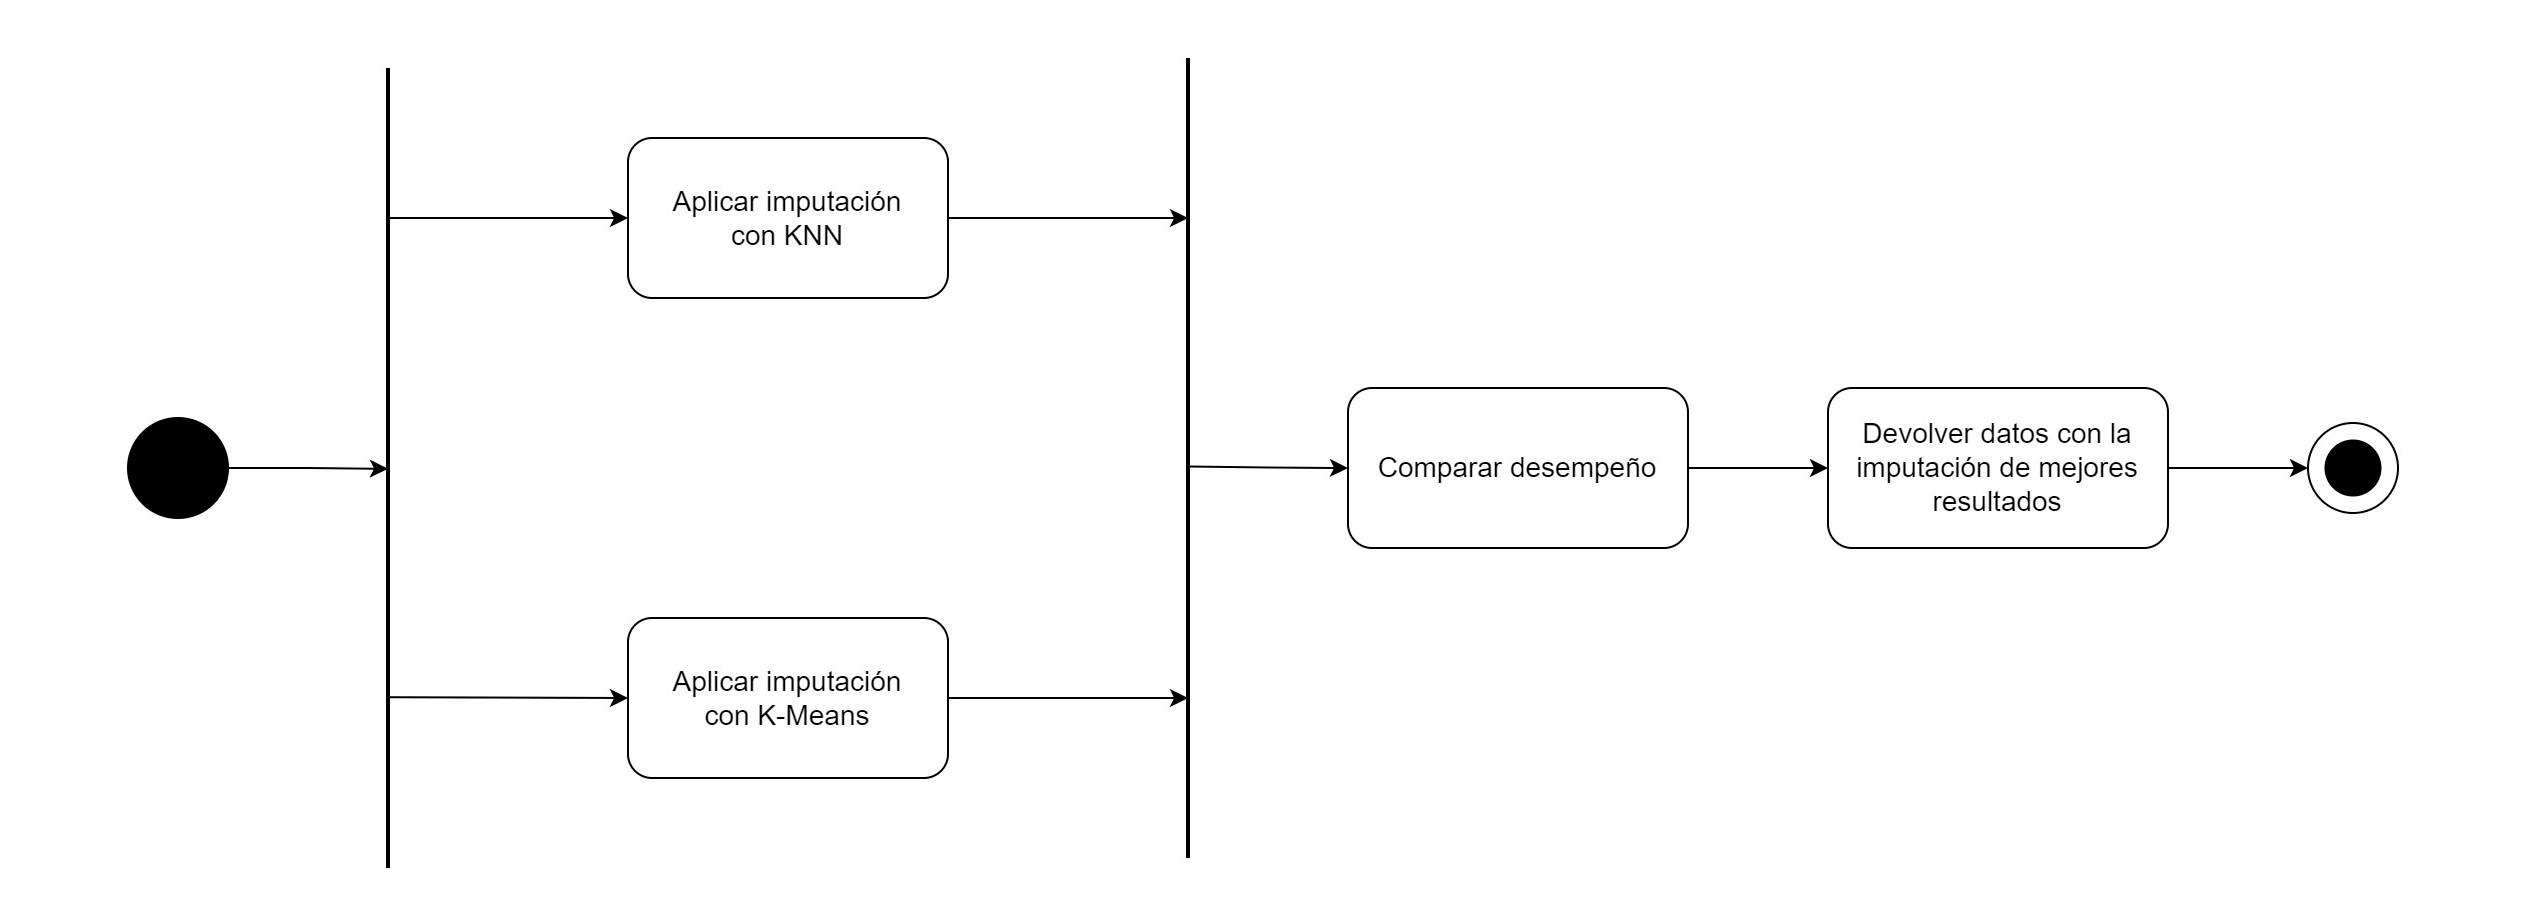
\includegraphics[width=1\linewidth]{"figuras/capi 2/preprocesado/mv imputation.drawio"}
	\caption{Diagrama de flujo para la imputación de valores faltantes}
	\label{fig:mv-imputation}
\end{figure}

Primeramente se aplican en paralelo las técnicas de imputación kNN y k-Means, al terminar se aplica el algoritmo de aprendizaje automático en cuestión con los datos imputados por cada método y, finalmente, se comparan los resultados acorde al esquema descrito en el subcomponente \textit{Discretizer} para devolver los datos con la mejor sustitución. \\
Para la implementación de kNN y k-Means, se crearon dos subcomponentes: kNN Imputation y kMI (K-Means Imputation). Se emplean los nodos \textit{kNN} y \textit{k-Means}, ambos nativos de KNIME. Para escoger \textit{k}, en k-Means se utiliza el método de la silueta, ya que KNIME contiene el nodo Silhouette Coefficient; mientras que para kNN se decide emplear la raíz cuadrada de la muestra, debido a su simpleza en la implementación. Además, este método podría ofrecer cierta estabilidad en la elección del número de vecinos, independientemente del tamaño específico del conjunto de datos. Esto podría hacer que el modelo sea menos sensible a variaciones en el tamaño de la muestra. A continuación se describe el funcionamiento de k-NNI y kMI:

\begin{itemize}
	\item kMI:
	\begin{enumerate}
		\item Convertir los valores nominales en numéricos para que el nodo trabaje con ellos, ya que este algoritmo solamente trata este tipo de valores.
		\item Separar las columnas con valores perdidos para que el algoritmo pueda realizar el proceso de clustering con los datos sin estos valores, ya que no los tolera el nodo.
		\item Calcular valor optimo de \textit{k} con el método de la silueta.
		\item Aplicar k-Means a estos datos.
		\item Unir las columnas que contienen valores perdidos con los datos etiquetados con su respectivo clúster.
		\item Aplicar el nodo \textit{Missing Value}, nativo de KNIME, tras filtrar por clúster, sustituyendo los valores perdidos por la media de esa columna, es decir el valor del centroide de ese clúster.
		\item Retornar las variables numéricas a categóricas (las que se transformaron inicialmente) para recuperar su valor original.
	\end{enumerate}
	\item kNNI:
	\begin{enumerate}
		\item Convertir los valores nominales en numéricos para que el nodo trabaje con ellos, ya que este algoritmo solamente trata este tipo de valores.
		\item Extraer los nombres de las columnas que contienen valores perdidas.
		\item Por cada columna, se separan los valores perdidos del resto de los datos, éstos se reemplazan por 0 si son numéricos, si son de tipo \textit{string} se ignoran.
		\item Calcular el valor de \textit{k} mediante la raíz cuadrada de la muestra. 
		\item Los datos sin valores perdidos se emplean para el entrenamiento de kNN, mientras los datos con estos se emplean para la predicción.
		\item Retornar las variables numéricas a categóricas (las que se transformaron inicialmente) para recuperar su valor original.
	\end{enumerate}
\end{itemize}

 En las figuras \ref{fig:flujo-knni} y \ref{fig:flujo-kmi} se muestran los flujos de trabajo que se implementan para la imputación con los algoritmos kNNI y kMI, respectivamente.
 
 \begin{figure}[H]
 	\centering
 	\includegraphics[width=0.9\linewidth]{"figuras/capi 2/preprocesado/flujo-knni"}
 	\caption{Vista previa de flujo KNIME para kNNI}
 	\label{fig:flujo-knni}
 \end{figure}
 
  \begin{figure}[H]
 	\centering
 	\includegraphics[width=0.9\linewidth]{"figuras/capi 2/preprocesado/flujo-kmi"}
 	\caption{Vista previa de flujo KNIME para kMI}
 	\label{fig:flujo-kmi}
 \end{figure}
 
 

\subsection{Codificación y normalización}
La codificación de variables categóricas implica asignar valores numéricos a estas categorías para que los algoritmos de aprendizaje automático puedan trabajar con ellas. Este es el propósito del subcomponente \textit{Pre-procesar números}, además de la normalización de variables numéricas. En aras de clarificar el funcionamiento de este proceso, se decide renombrarlo a \textit{Codificar y normalizar}.\\
La normalización son proporciones sin unidades de medida (adimensionales o invariantes de escala) que nos permiten poder comparar elementos de distintas variables y unidades de medida. Esta es necesaria para cambiar los valores de las columnas numéricas del conjunto de datos para usar una escala común, sin distorsionar las diferencias en los intervalos de valores ni perder información. La normalización es fundamental para que algunos algoritmos modelen los datos correctamente. \\
En KNIME es posible implementar la normalización a partir del nodo \textit{Normalizer}. En este nodo se encuentran tres métodos para normalizar, a elección del usuario: \textit{Decimal Scaling, Z-Score y Min-Max}. Este proceso se encuentra en el subcomponente para el pre-procesado de números, cuyo diagrama de flujo se presenta en la figura \ref{fig:number-preprocs}. \\
Por otro lado, los valores de alta cardinalidad, aquellos que se repiten con frecuencia y pueden ser numerosos, son cruciales para comprender tendencias y patrones en los datos. La codificación de estas variables se refiere a técnicas especiales de codificación que se utilizan cuando se tienen variables categóricas con un gran número de categorías o niveles distintos. La alta cardinalidad puede dificultar la gestión de estas variables en modelos de aprendizaje automático, y es importante abordarlas de manera eficiente. \\

\begin{figure}[H]
	\centering
	\includegraphics[width=1\linewidth]{"figuras/capi 2/preprocesado/number preprocs.drawio"}
	\caption{Diagrama de flujo del pre-procesado para la codificación y normalización}
	\label{fig:number-preprocs}
\end{figure}

A continuación se exponen los cambios realizados al pre-procesado para la codificación y normalización:

\begin{itemize}

	\item Codificar con One-Hot Encoding: para el tratamiento de valores con alta cardinalidad, se emplea la codificación One-Hot (ver epígrafe \ref{alta-cardinalidad}), ya que KNIME brinda el nodo \textit{One To Many} para esta tarea. Para esto se escogen los atributos que tienen como mínimo 15 categorías distintas. One-Hot Encoding se utiliza para codificar variables categóricas en una forma que no impone un orden implícito en las categorías. Cuando se tienen más de 15 categorías, es poco probable que haya un orden natural o jerarquía en esas categorías, por lo que codificarlas como variables binarias evita interpretaciones erróneas de orden o importancia. Dado que esta técnica produce gran dimensionalidad, se utiliza para su reducción el método PCA, con un límite de conservación de la información del 90\%. Este proceso se encuentra implementado en la figura \ref{fig:one-hot-flujo}.
	
	\begin{figure}[H]
		\centering
		\includegraphics[width=0.9\linewidth]{"figuras/capi 2/preprocesado/one-hot-flujo"}
		\caption{Vista previa de flujo KNIME para codificacion One-Hot}
		\label{fig:one-hot-flujo}
	\end{figure}
	
	\item Normalizar: en aras de automatizar este proceso, se propone el subcomponente \textit{Normalizer}, de igual nombre al nodo nativo de KNIME, en donde se encuentra el mismo para la ejecución de los métodos que contiene, en función de un modelo predeterminado. En la figura \ref{fig:normalizacion} se presenta el diagrama de flujo de este subcomponente. 

\end{itemize}

\begin{figure}[H]
	\centering
	\includegraphics[width=1\linewidth]{"figuras/capi 2/preprocesado/normalizacion.drawio"}
	\caption{Diagrama de flujo para la normalización}
	\label{fig:normalizacion}
\end{figure}

Siguiendo el mismo esquema del subcomponente \textit{Discretizer}, tras aplicar la normalización con los distintos métodos ofrecidos por la herramienta KNIME, se aplica el algoritmo de aprendizaje automático que requiere los datos normalizados y posteriormente, se realiza la evaluación del desempeño de cada uno, acorde a las métricas Precisión y Cohen's Kappa. Luego de escoger el mejor, se devuelve la tabla con los datos normalizados.


\section{Componente AutoML Clasificación (Optimización de hiperparámetros)}
Antes de explorar en detalle las adaptaciones realizadas en cada modelo, es fundamental presentar un nuevo componente para la optimización de hiperparámetros, con el objetivo de facilitar el entendimiento en los epígrafes posteriores. \\
Los modelos a optimizar en el componente propuesto en este acápite, se derivan del componente \textit{AutoML Clasificación (pre-procesado)}, dichos modelos son: redes neuronales mediante retropropagación (RProp), redes neuronales probabilísticas (PNN) y máquinas de soporte vectorial (SVM). Es importante señalar que, a diferencia del componente \textit{AutoML Clasificación (pre-procesado)}, no se incorporan los modelos ID3, CART y C4.5. Esto se debe a que no permiten la optimización de hiperparámetros, ya que son nodos de la extensión KNIME WEKA, que carecen de configuración de variables de flujo. Por esta razón, se ha tomado la decisión de implementar otra variante: Random Forest. \\
La selección adecuada de variables desempeña un papel fundamental en el desarrollo de modelos de aprendizaje automático y estadísticos. Las variables que se incluyen en un modelo no solo afectan su capacidad para comprender patrones y tomar decisiones precisas, sino que también pueden influir significativamente en la eficiencia computacional y los recursos requeridos. Al elegirlas correctamente, se simplifica y mejora la interpretación de los modelos, reduce el riesgo de sobreajuste y acelera el tiempo de entrenamiento. Algunas variables que influyen en el rendimiento de los modelos son: 
\begin{itemize}
	\item Random Forest: Número de árboles en el bosque, criterio de división, profundidad máxima, número mínimo de muestras requeridas para dividir un nodo, peso asignado a las clases en el conjunto de datos, número mínimo de muestras requeridas para estar en un nodo hoja.
	
	\item SVM: Tipo de kernel, número máximo de iteraciones, parámetro de regularización, pesos a las clases, sesgo de la ecuación del hiperplano.
	
	\item Redes Neuronales por Retropropagación: Tasa de aprendizaje, número de épocas, número de capas, cantidad de neuronas por capa, inicialización de pesos, regularización.
	
	\item Redes Neuronales Probabilísticas: Conexión sináptica entre dos neuronas, tasa de aprendizaje, número de épocas, número de capas y la cantidad de neuronas por capa.
\end{itemize}

Es importante destacar que la selección de variables debe basarse en un conocimiento sólido del problema en cuestión y en un análisis cuidadoso de su impacto en la calidad y eficacia del modelo. La selección de variables a optimizar por algoritmo se desarrolla en los epígrafes posteriores. \\
Ajustar las configuraciones de un modelo es clave para lograr un rendimiento óptimo, lo que a su vez mejora la precisión y la eficacia de sus análisis. En este contexto, se propone el componente \textit{AutoML Clasificación (Optimización de hiperparámetros)},  presente en la figura \ref{fig:automl-componente-hpo}, conteniendo la siguiente configuración:

\begin{figure}[H]
	\centering
	\includegraphics[width=0.35\linewidth]{"figuras/capi 2/hpo/automl-componente-hpo"}
	\caption[Componente AutoML Clasificación (Optimización de Hiperparámetros)]{Componente \textit{AutoML Clasificación (Optimización de Hiperparámetros)}}
	\label{fig:automl-componente-hpo}
\end{figure}
\begin{enumerate}
	\item Puerto de entrada: recibe los datos de entrada en formato tabular.
	\item Elementos de la configuración:
	\begin{itemize}
		\item Selección de modelos: Lista de modelos a entrenar y optimizar disponibles (Redes Neuronales por Retropropagación, Redes Neuronales Probabilísticas, Random Forest y SVM).
		\item Selección de porcentaje de la partición de entrenamiento: el valor introducido determina el factor en que se divide el conjunto de datos para entrenar y probar cada algoritmo, selección disponible en un rango de 1 a 99. 
		\item Columna objetivo: presenta las columnas de tipo \textit{string} que pueden fungir como columna objetivo.
		\item Estrategia de optimización de hiperparámetros: se selecciona la estrategia de optimización de hiperparámetros entre las disponibles (Random Search, Bayesian Optimization (TPE), Brute Force y Hillclimbing).
		\item Selección del número de subconjuntos de la validación cruzada: el valor introducido determina la cantidad de veces que se divide el conjunto de datos en subconjuntos de entrenamiento y prueba, durante el proceso de validación.
	\end{itemize}
	\item Puerto de salida: tabla de selección múltiple de modelos con hiperparámetros optimizados.
\end{enumerate}

\begin{comment}
	
\subsection{Uso y configuración del componente AutoML Clasificación (Optimización de Hiperparámetros)}
A continuación, se define la secuencia de pasos para el correcto funcionamiento del componente \textit{AutoML Clasificación (Optimización de Hiperparámetros)}:

\begin{enumerate}
	\item Proporcionar el conjunto de datos al puerto de entrada (el componente marcará error en este punto, pues la configuración es obligatoria).
	\item Dar click derecho sobre el componente, seleccionar “Configure…”. 
	\item Seleccionar la configuración deseada (como se observa en el ejemplo de la figura \ref{fig:config-automl-hpo}). 
	\item Ejecutar el componente (inicialmente el puerto de salida se encuentra vacío).
	\item Dar click derecho sobre el componente y seleccionar “Interactive View: AutoML” (Fig3). 
\end{enumerate}

\begin{figure}[H]
	\centering
	\includegraphics[width=0.5\linewidth]{"figuras/capi 2/config-automl-hpo"}
	\caption[Ejemplo de configuración del componente AutoML (Optimización de Hiperparámetros)]{Ejemplo de configuración del componente \textit{AutoML (Optimización de Hiperparámetros)}}
	\label{fig:config-automl-hpo}
\end{figure}

\begin{figure}[H]
	\centering
	\includegraphics[width=0.5\linewidth]{"figuras/capi 2/automl-hpo-vista-salida"}
	\caption[Vista de la salida.]{Vista de la salida.}
	\label{fig:automl-hpo-vista-salida}
\end{figure}

\end{comment}


\subsection{Requisitos y restricciones del componente AutoML Clasificación (Optimización de Hiperparámetros)}
El componente propuesto debe cumplir los siguientes requisitos funcionales:

\begin{itemize}
	\item RF1: El componente debe permitir seleccionar columna objetivo
	\item RF2: El componente debe permitir seleccionar estrategia de optimización de hiperparámetros.
	\item RF3: El componente debe permitir seleccionar cantidad de subconjuntos en la validación cruzada.
	\item RF4: El componente debe permitir seleccionar uno o varios de los algoritmos listados.
	\item RF5: El componente debe permitir seleccionar el porcentaje de la partición de entrenamiento.
	\item RF6: El componente debe entrenar y optimizar hiperparámetros para Redes Neuronales de Retropropagación. 
	\item RF7: El componente debe entrenar y optimizar hiperparámetros para Redes Neuronales Probabilísticas. 
	\item RF8: El componente debe entrenar y optimizar hiperparámetros para SVM.
	\item RF9: El componente debe entrenar y optimizar hiperparámetros para Random Forest.
	\item RF10: El componente debe graficar los modelos seleccionados.
	\item RF11: El componente debe retornar el modelo seleccionado por el usuario.
\end{itemize}

El componente propuesto presenta las siguientes restricciones para su funcionamiento:

\begin{itemize}
	\item Los datos de entrada deben encontrarse en formato tabular.
	\item La columna objetivo debe ser de tipo \textit{string}.
	\item Los datos numéricos deben estar previamente normalizados.
\end{itemize}

\subsection{Modelación del componente AutoML Clasificación (Optimización de Hiperparámetros)}
El diagrama de flujo de la figura \ref{fig:diagrama-flujo-gral-comp-hpo} expone el flujo general del componente \textit{AutoML Clasificación (Optimización de Hiperparámetros)}.

\begin{figure}[h]
	\centering
	\includegraphics[width=1\linewidth]{"figuras/capi 2/hpo/diagrama-flujo-gral-comp-hpo"}
	\caption[Diagrama de flujo general del componente AutoML Clasificación (Optimización de Hiperparámetros)]{Diagrama de flujo general del componente \textit{AutoML Clasificación (Optimización de Hiperparámetros)}}
	\label{fig:diagrama-flujo-gral-comp-hpo}
\end{figure}

En la fase inicial, se procede a la definición de la configuración de parámetros, durante la cual se especifican las variables determinantes que guiarán el flujo de ejecución del proceso. Luego, se procede con la optimización de los hiperparámetros de los modelos seleccionados por el usuario, lo que da como resultado la generación de los modelos que serán representados gráficamente. Según si la columna objetivo presenta múltiples clases o no, se realizan las representaciones gráficas de los modelos y se otorga al usuario la capacidad de elegir aquel que mejor concuerde con sus requisitos particulares.

\subsubsection*{Selección de parámetros}
Los parámetros que rigen el funcionamiento del componente propuesto, brindan al usuario una mayor personalización de la optimización de hiperparámetros, pues le ofrece la libertad de configurar múltiples factores claves de esta etapa. El diagrama de actividades de la figura \ref{fig:diagrama-act-selecc-param-hpo} expone el flujo para la selección de parámetros.

\begin{figure}[H]
	\centering
	\includegraphics[width=0.7\linewidth]{"figuras/capi 2/hpo/diagrama-act-selecc-param-hpo"}
	\caption[Diagrama de actividades de selección de parámetros]{Diagrama de actividades de selección de parámetros}
	\label{fig:diagrama-act-selecc-param-hpo}
\end{figure}

La selección de parámetros se realiza con los siguientes nodos de configuración, presentes en el repositorio base:

\begin{itemize}
	\item Seleccionar columna objetivo: se emplea el nodo \textit{Column Selection Configuration}, el cual recibe una tabla y devuelve el nombre de la columna seleccionada como variable de flujo. En este caso, presenta la configuración adicional para solo mostrar las columnas de tipo \textit{string}.
	\item Seleccionar estrategia de optimización de hiperparámetros: la selección de la estrategia se lleva a cabo empleando el nodo \textit{Single Selection Configuration}. Devuelve la variable \texttt{strategy} con el valor seleccionado previamente.
	\item Seleccionar número de subconjuntos en la validación cruzada: la selección de la cantidad de subconjuntos de partición de entrenamiento se lleva a cabo con el nodo \textit{Integer Configuration}. Este devuelve la variable de flujo resultante de la selección, en este caso presenta la configuración para limitar el rango entre 5 y 10.  La selección de la partición de entrenamiento se lleva a cabo con el mismo nodo anteriormente mencionado.
	\item Evaluar columna objetivo: se evalúa en clase binaria o multiclase la columna objetivo mediante los nodos listados en la \textbf{fig *** (Foto para anexos) }
	\item Seleccionar modelo o modelos a optimizar: la selección se realiza mediante el nodo \textit{Multiple Selection Configuration}, el cual devuelve la variable \texttt{modelo} con la selección.
\end{itemize}

\subsubsection*{Optimización de hiperparámetros}
El diagrama de flujo de la figura \ref{fig:optimizacion-a-resumen-2} expone el flujo general del apartado de optimización del componente \textit{AutoML Clasificación (Optimización de Hiperparámetros)}.

\begin{figure}[H]
	\centering
	\includegraphics[width=1\linewidth]{"figuras/capi 2/hpo/Optimizacion a resumen 2.14"}
	\caption{Diagrama de flujo de la optimización de hiperparámetros}
	\label{fig:optimizacion-a-resumen-2}
\end{figure}

En la figura \ref{fig:optimizacion-a-resumen-2}, la optimización de hiperparámetros implica la iteración sistemática a través de un conjunto predefinido de hiperparámetros, evaluando exhaustivamente todas las combinaciones posibles. Este proceso se detiene una vez que se han evaluado todas las combinaciones. Cada iteración se somete a una validación cruzada, que implica la evaluación de los hiperparámetros en múltiples subconjuntos de prueba. La métrica de rendimiento (en este caso, la exactitud) se calcula para cada iteración de la validación cruzada, y se registra la iteración con la mayor exactitud. Finalmente, una vez que se han evaluado todas las combinaciones posibles, se devuelve la iteración del modelo que obtuvo la mejor exactitud. \\
En KNIME es posible implementar el ciclo para comprobar las combinaciones de hiperparámetros mediante los nodos \textit{Parameter Optimization Loop Start} y \textit{Parameter Optmization Loop End}, los cuales permiten almacenar las iteraciones realizadas por el algoritmo con las diferentes combinaciones de hiperparámetros dentro de un rango previamente establecido. En el \textbf{anexo ****} se muestra el flujo correspondiente al funcionamiento genérico de un flujo de optimización.

\subsubsection*{Graficar y seleccionar modelos}
Una parte esencial de cualquier flujo de trabajo en KNIME es la etapa en la que se exploran, comparan y seleccionan los modelos. Esta fase se convierte en el núcleo de la toma de decisiones en la analítica de datos, ya que permite identificar cuál de los modelos propuestos se ajusta de manera óptima a los datos y objetivos.
KNIME brinda herramientas para visualizar y evaluar el rendimiento de los modelos, lo que permite tomar decisiones informadas y seleccionar el modelo que mejor se adapte a las necesidades del usuario. En el proceso de modelado y selección, se emplean los nodos \textit{Binary Classification Inspector} y \textit{ROC Curve} para problemas de clasificación binaria \textbf{fig*} y, en cambio, se utilizan los nodos \textit{Bar Chart} y \textit{Table View} cuando se enfrentan problemas de clasificación multiclase \textbf{fig*. (Las figuras de anexo q serian flujos)}


\subsection{Optimización de hiperparámetros para RProp}
Para el entrenamiento y prueba de las Redes Neuronales por Retropropagación, se emplean los nodos \textit{RProp MLP Learner} y \textit{MultiLayerPerceptron Predictor}, donde debido a las limitaciones de KNIME y su importancia en el rendimiento del modelo se seleccionan los hiperparámetros a optimizar siguientes:
	\begin{enumerate}
		\item \textit{Número máximo de iteraciones:} Generalmente llamado "número de épocas" (number of epochs), se define como un pase completo a través de todo el conjunto de datos durante el proceso de entrenamiento. Es un hiperparámetro crítico que controla cuántas veces la red pasará por el conjunto de datos de entrenamiento para ajustar sus pesos y mejorar su rendimiento. \textbf{Esta variable se comparte para el algoritmo Redes Neuronales Probabilísticas} \citep{montavon2012neural}.
		\item \textit{Cantidad de neuronas:} Número de neuronas o unidades en una capa específica de una red neuronal, afecta la capacidad de la red para aprender y representar patrones complejos en los datos \citep{montavon2012neural}.
		\item \textit{Número de capas:} Número de capas ocultas que se encuentran entre la capa de entrada y la capa de salida de la red. Estas se utilizan para aprender y representar patrones y características en los datos de entrada \citep{montavon2012neural}.
	\end{enumerate}

El diagrama de actividades de la figura \ref{fig:optimizacion-rprop}, expone el flujo para el procesamiento necesario para la ejecución del algoritmo Redes Neuronales por Retropropagación, con optimización de hiperparámetros.

\begin{figure}[H]
	\centering
	\includegraphics[width=1\linewidth]{"figuras/capi 2/hpo/Optimizacion RProp"}
	\caption{Diagrama de flujo para la optimización de hiperparámetros de RProp}
	\label{fig:optimizacion-rprop}
\end{figure}


\subsection{Optimización de hiperparámetros para PNN}
En el contexto del algoritmo de Redes Neuronales Probabilísticas (PNN), se hacen uso de dos nodos: \textit{PNN Learner} y \textit{PNN Predictor}. Estos nodos son utilizados para configurar y ejecutar el algoritmo, y se enfocan en la selección y optimización de diversas variables críticas. En particular, debido a las limitaciones de KNIME se ajustan los siguientes hiperparámetros:

	\begin{enumerate}
		\item \textit{Theta Minus ($\theta$-):} Representa la disminución de la fuerza de una conexión sináptica entre dos neuronas. Si dos neuronas están activas simultáneamente con frecuencia baja, la conexión sináptica entre ellas disminuirá, lo que se conoce como "depresión sináptica". Se usa para evitar que las conexiones se fortalezcan en exceso y se vuelvan saturadas \citep{montavon2012neural}.
		\item \textit{Theta Plus ($\theta$+):} Representa el aumento de la fuerza de una conexión sináptica entre dos neuronas. Si dos neuronas están activas juntas con frecuencia alta, la conexión entre ellas se fortalecerá, lo que se conoce como "potenciación sináptica". Esto ayuda a fortalecer las conexiones que son relevantes \citep{montavon2012neural}.
\end{enumerate}

Estos parámetros son esenciales para el rendimiento y la convergencia del algoritmo. El diagrama de actividades representado en la figura \ref{fig:optimizacion-pnn} proporciona una visualización estructurada del flujo de procesos y operaciones, necesarios para la ejecución del algoritmo de Redes Neuronales por Retropropagación con un enfoque específico en la optimización de hiperparámetros.

\begin{figure}[H]
	\centering
	\includegraphics[width=1\linewidth]{"figuras/capi 2/hpo/Optimizacion PNN"}
	\caption{Diagrama de flujo para la optimización de hiperparámetros de PNN}
	\label{fig:optimizacion-pnn}
\end{figure}


\subsection{Optimización de hiperparámetros para SVM}

Para la Máquina de Soporte Vectorial (SVM), se realiza la selección de los hiperparámetros siguientes:

	\begin{enumerate}
		\item \textit{Kernels:} función matemática que se utiliza para realizar una transformación no lineal de los datos de entrada. Permiten la clasificación efectiva de datos que no son linealmente separables en el espacio de características original. Mapean los datos a un espacio de características de mayor dimensión donde es más probable que sean linealmente separables \citep{scholkopf2018learning}, \citep{bishop2006pattern}. En esta investigación se utilizan tres tipos de kernels \citep{scholkopf2018learning}:
		\begin{enumerate}
			\item \textit{RBF:} Utiliza una función gaussiana para mapear los datos en un espacio de características de mayor dimensión, lo que es útil para problemas de clasificación no lineales.
			\item \textit{Polinómico:} Transforma los datos utilizando funciones polinómicas, adecuado para problemas donde los datos pueden ser separados por una frontera polinómica.
			\item \textit{Hiperbólico tangente:} Utiliza la función tangente hiperbólica para realizar la transformación no lineal de los datos.
		\end{enumerate}
		\item \textit{Bias:} sesgo de la ecuación del hiperplano de decisión, controla la posición del hiperplano y asegura que se ajuste adecuadamente entre las clases en un problema de clasificación \citep{scholkopf2018learning}, \citep{joachims2002learning}.
		\item \textit{Gamma:} El parámetro gamma controla la flexibilidad del modelo y la capacidad de ajustar los datos. Los valores bajos de gamma indican un gran radio de similitud, que da como resultado que se agrupen más puntos; mientras que los valores altos de gamma indican un radio de similitud más pequeño y una mayor complejidad del modelo  \citep{bishop2006pattern}, \citep{scholkopf2018learning}.
	\end{enumerate}


El proceso se encuentra representado en un diagrama de flujo, como se ilustra en la figura \ref{fig:optimizacion-svm}. Este diagrama de flujo proporciona una visión general de cómo se lleva a cabo la optimización de SVM, detallando el flujo de decisiones y operaciones involucradas en la selección del kernel y sus hiperparámetros correspondientes.

\begin{figure}[H]
	\centering
	\includegraphics[width=1\linewidth]{"figuras/capi 2/hpo/Optimizacion SVM"}
	\caption{Diagrama de flujo para la optimización de hiperparámetros de SVM}
	\label{fig:optimizacion-svm}
\end{figure}


\subsection{Optimización de hiperparámetros para Random Forest}
En el marco de la implementación de Random Forest, se hacen uso de los nodos \textit{Random Forest Learner} y \textit{Random Forest Predictor}, donde se seleccionan los hiperparámetros a optimizar:

	\begin{enumerate}
	\item \textit{Profundidad máxima:} Es la profundidad de los árboles en el bosque. Controla la cantidad de niveles o divisiones que tiene desde el nodo raíz hasta las hojas y ayuda a evitar el sobreajuste \citep{lakshmanan2021practical}, \citep{hastie2009elements}.
	\item \textit{Cantidad de modelos:} Cantidad de árboles de decisión que se construyen en el bosque aleatorio. Cada árbol se entrena en una submuestra aleatoria del conjunto de datos de entrenamiento. Aumentar su valor generalmente hace que el modelo sea más robusto y preciso, pero también puede aumentar el costo computacional \citep{lakshmanan2021practical}.
	\item \textit{Tamaño mínimo del nodo:} Establece un límite en la cantidad mínima de ejemplos necesarios en un nodo para que se considere una división. Si el número de ejemplos en un nodo es menor que el valor especificado, no se realizará una división en ese nodo, lo que ayuda a evitar una partición excesiva y a reducir la complejidad del árbol \citep{lakshmanan2021practical}.
	\item \textit{Criterio de división:} medida utilizada para evaluar la calidad de una partición en un nodo del árbol. Determina cómo se eligen las características para dividir los nodos. En la presente investigación se tratan tres criterios de división \citep{gupta2017analysis}:
	\begin{enumerate}
		\item Ganancia de Información (Information Gain): evalúa cómo una división particular afecta la entropía o la impureza del conjunto de datos. Al seleccionar la característica que maximiza la ganancia de información, se elige la división que proporciona la mayor claridad en términos de la distribución de las clases en los nodos hijos. 
		\item Gini Index: cuantifica qué tan a menudo un elemento seleccionado al azar sería incorrectamente etiquetado. Minimizar su valor durante la construcción del árbol lleva a la creación de nodos donde la probabilidad de error de clasificación es más baja. 
		\item Radio de Ganancia de Información (Information Gain Ratio): ajusta la ganancia de información dividiéndola por la información intrínseca de la característica. Esto promueve la selección de características que no solo ofrecen alta ganancia de información, sino que también tienen información intrínseca moderada. 
	\end{enumerate}
\end{enumerate}

La figura \ref{fig:optimizacion-randomforest} brinda una representación organizada del flujo de procesos y operaciones necesarias para la ejecución de la optimización del algoritmo Random Forest, detallando la selección del criterio de división de Random Forest.


\begin{figure}[H]
	\centering
	\includegraphics[width=1\linewidth]{"figuras/capi 2/hpo/Optimizacion RandomForest"}
	\caption{Diagrama de flujo para la optimización de hiperparámetros de Random Forest}
	\label{fig:optimizacion-randomforest}
\end{figure}


\section{Modelación de nueva versión del componente AutoML Clasificación}
El enfoque principal de esta propuesta es la integración de los subcomponentes desarrollados para el pre-procesado y el componente \textit{AutoML Clasificación (Optimización de hiperparámetros)} con el componente AutoML existente para clasificación, cuyo diagrama de flujo se presenta en la figura \ref{fig:diagrama-general-componente}. \\

\begin{figure}[H]
	\centering
	\includegraphics[width=0.9\linewidth]{"figuras/capi 2/Diagrama General Componente"}
	\caption{Diagrama de flujo de Componente AutoML (clasificación)}
	\label{fig:diagrama-general-componente}
\end{figure}

Como se puede apreciar en la figura \ref{fig:diagrama-general-componente}, se implementa un nuevo modelo para la clasificación: Random Forest. Además, se realizan cambios en la personalización del componente: la eliminación del umbral de valores únicos por columna y un nuevo campo para la elección de la estrategia de optimización que se utilizará para la optimización de hiperparámetros. Con el propósito de abordar la integración con las nuevas implementaciones, se discutirán detalladamente en las secciones siguientes.

\subsection{Procesado de ID3}
El algoritmo ID3 se puede ejecutar en KNIME a través del nodo \textit{Id3 (3.7)}, el cual forma parte de una extensión de la herramienta Weka. Al no ser un nodo nativo en KNIME, no es posible optimizar los hiperparámetros del mismo, sin embargo se realizaron las integraciones con los subcomponentes de pre-procesado discutidos en las secciones anteriores. Esto se manifiesta en el diagrama de flujo presente en la figura \ref{fig:procesado-id3}.

\begin{figure}[H]
	\centering
	\includegraphics[width=0.9\linewidth]{"figuras/capi 2/modelos/procesado id3.drawio"}
	\caption{Diagrama de flujo del procesamiento del modelo ID3}
	\label{fig:procesado-id3}
\end{figure}

Tal como se puede apreciar en la figura \ref{fig:procesado-id3}, simplemente se realizaron las modificaciones pertinentes en el manejo de valores faltantes, la discretización y el pre-procesado de \textit{string}. No se incorpora la codificación y normalización, dado que este algoritmo no tolera variables numéricas.

\subsection{Procesado para C4.5}
El algoritmo C4.5 puede ejecutar en KNIME a traves del nodo \textit{J48}. Este, al igual que Id3, forma parte de la extensión Weka y no permite la incorporación de la optimización de hiperparámetros. Las modificaciones efectuadas en el pre-procesado están presentes en el diagrama de flujo de la figura \ref{fig:procesado-c4pt5}.

\begin{figure}[h]
	\centering
	\includegraphics[width=1\linewidth]{"figuras/capi 2/modelos/procesado c4pt5.drawio"}
	\caption{Diagrama de flujo del procesamiento del modelo C4.5}
	\label{fig:procesado-c4pt5}
\end{figure}

Como se observa, estas modificaciones fueron las mismas que a su predecesor, con la diferencia de que, en la versión anterior del componente \textit{AutoML Clasificación (pre-procesado)}, en este modelo no estaba presente la discretización, ya que es un algoritmo versátil y puede manejar tanto variables categóricas como numéricas. Sin embargo, se decide incorporarla ya que, a pesar de lo anteriormente expuesto, C4.5 puede ser menos eficaz cuando se utiliza en conjuntos de datos con datos numéricos muy dispersos. En tales casos, los árboles de decisión pueden requerir una mayor profundidad para capturar patrones en las variables numéricas, lo que puede llevar a árboles más complejos y propensos al sobreajuste. 

\subsection{Procesado para CART}
El algoritmo CART tiene los mismos requisitos que C4.5 para su ejecución, por lo que la diferencia entre ambos es el nodo que ejecuta el algoritmo, pues emplea el nodo \textit{SimpleCart (3.7)}. La única diferencia es que no se emplea la discretización de variables numéricas, ya que este árbol de decisión puede ser empleado tanto en tareas de clasificación como de regresión, lo que provoca que funcione de manera efectiva tanto con datos numéricos como nominales. Por otra parte, al formar parte de la extensión Weka, este nodo tampoco presenta la optimización de hiperparámetros. \\
En la figura \ref{fig:procesado-cart} se presenta el diagrama de flujo del procesado del algoritmo CART.

\begin{figure}[H]
	\centering
	\includegraphics[width=1\linewidth]{"figuras/capi 2/modelos/procesado cart.drawio"}
	\caption{Diagrama de flujo del procesado de CART}
	\label{fig:procesado-cart}
\end{figure}


\subsection{Procesamiento para Random Forest}
Dado que los modelos de árboles de decisión empleados en el componente \textit{AutoML Clasificación (pre-procesado)} forman parte de extensiones Weka y, por tal motivo, no se puede ejecutar la optimización de hiperparámetros, se decide agregar un nuevo modelo: Random Forest. Este algoritmo puede trabajar con una amplia variedad de tipos de datos, ya sean datos numéricos o categóricos. Esto hace que Random Forest sea una elección versátil para tareas de clasificación y regresión. Por ello, el pre-procesado de este algoritmo es igual al de CART. \\
El diagrama de flujo del procesado de este nuevo modelo se muestra en la figura \ref{fig:procesado-rf}.

\begin{figure}[H]
	\centering
	\includegraphics[width=1\linewidth]{"figuras/capi 2/modelos/procesado rf.drawio"}
	\caption{Diagrama de flujo del procesamiento de Random Forest}
	\label{fig:procesado-rf}
\end{figure}


\subsection{Procesamiento para Redes Neuronales por Retropropagación}
Las Redes Neuronales por Retropropagación necesitan procesar los valores numéricos, además de los procesamientos realizados para C4.5 y CART, dado que solo permiten atributos de ese tipo. Por esta razón, se incluye el subcomponente para la codificación y normalización, tal como se muestra en el diagrama de flujo de la figura \ref{fig:procesado-rprop}. Este algoritmo tiene la restricción de que solo se admiten valores entre 0 y 1, por tanto solo se realizan las normalizaciones Min-Max y Decimal Scaling. Por otra parte, también se implementa la optimización de hiperparámetros al integrar el componente \textit{AutoML Clasificación (Optimización de hiperparámetros)}.

 \begin{figure}[H]
	\centering
	\includegraphics[width=1\linewidth]{"figuras/capi 2/modelos/procesado rprop.drawio"}
	\caption{Diagrama de flujo del procesamiento de RProp}
	\label{fig:procesado-rprop}
\end{figure}



\subsection{Procesamiento para Redes Neuronales Probabilísticas}
Las Redes Neuronales Probabilísticas, al igual que RProp, trabajan con atributos numéricos. Por ello, se decide incorporar la codificación y normalización, la cual estaba en la versión anterior, sin embargo la normalización no se encontraba. Como en RProp, se implementa la optimización de hiperparámetros al integrar el componente \textit{AutoML Clasificación (Optimización de hiperparámetros)}. En la figura \ref{fig:procesado-pnn} se muestra el diagrama de flujo de procesamiento de PNN.

\begin{figure}[H]
	\centering
	\includegraphics[width=1\linewidth]{"figuras/capi 2/modelos/procesado pnn.drawio"}
	\caption{Diagrama de flujo para el procesado de PNN}
	\label{fig:procesado-pnn}
\end{figure}


\subsection{Procesamiento para SVM}
En este algoritmo, al igual que en las redes neuronales, se trabaja con atributos numéricos. No obstante, como fue el caso de PNN, no se encontraba la normalización de variables numéricas, que a pesar de no ser un requisito por el algoritmo, es un paso clave para su desempeño. Por otra parte, se implementa la optimización de hiperparámetros al integrar el componente \textit{AutoML Clasificación (Optimización de hiperparámetros).} El diagrama de flujo para el procesamiento de SVM se muestra en la figura \ref{fig:procesado-svm}.

\begin{figure}[H]
	\centering
	\includegraphics[width=1\linewidth]{"figuras/capi 2/modelos/procesado svm.drawio"}
	\caption{Diagrama de flujo del procesamiento de SVM}
	\label{fig:procesado-svm}
\end{figure}


\section{Conclusiones parciales}
En el Capítulo \ref{chap:2}, se presentaron una serie de modificaciones destinadas a mejorar el componente de \emph{AutoML Clasificación (pre-procesado)}. Estas modificaciones se centraron en el pre-procesamiento de datos y la optimización de hiperparámetros, con el objetivo de crear un sistema más eficiente y preciso para la construcción de modelos de clasificación. El enfoque principal de dichas propuestas fue la integración de estas mejoras con el componente AutoML existente, con el fin de proporcionar modelos de clasificación adaptados a las necesidades específicas de los datos.\\
A partir de lo analizado en este capítulo, se arriba a las siguientes conclusiones:
\begin{itemize}
	\item Se obtiene el diseño de un subcomponente para la discretización de variables numéricas.
	\item Para la discretización, se implementan los métodos Equal-Width, Equal-Frequency, Quantile-Based y CAIM.
	\item La implementación de los métodos de discretización se realiza con los nodos nativos de KNIME \textit{Auto-Binner} y \textit{CAIM Binner}.
	\item Se obtiene el diseño del componente AutoML Clasificación (Optimización de hiperparámetros).
	\item Se describe el uso y  los diferentes requisitos y restricciones del componente AutoML Clasificación (Optimización de hiperparámetros).
	\item Se define el rango de hiperparámetros (Iteraciones, capas y número de neuronas) del algoritmo Rprop.
\end{itemize}

\pagebreak

